\documentclass[]{interim_report}
\usepackage{graphicx}
\usepackage{hyperref}
\usepackage{longtable}
\usepackage{mathtools}


%%%%%%%%%%%%%%%%%%%%%%
%%% Input project details
\def\studentname{Eman Naveed}
\def\reportyear{2024}
\def\projecttitle{Lindenmayer Systems}
\def\supervisorname{Anand Subramoney}
\def\degree{MSci (Hons) in Computer Science}
\def\fullOrHalfUnit{Full Unit} % indicate if you are doing the project as a Full Unit or Half Unit
\def\finalOrInterim{Interim Report} % indicate if this document is your Final Report or Interim Report

\begin{document}

\maketitle

%%%%%%%%%%%%%%%%%%%%%%
%%% Declaration

\chapter*{Declaration}

This report has been prepared on the basis of my own work. Where other published and unpublished source materials have been used, these have been acknowledged.

\vskip3em

Word Count: 3826

\vskip3em

Student Name: \studentname

\vskip3em

Date of Submission: December 13, 2024

\vskip3em

Signature: Eman Naveed

\newpage

%%%%%%%%%%%%%%%%%%%%%%
%%% Table of Contents
\tableofcontents\pdfbookmark[0]{Table of Contents}{toc}\newpage

%%%%%%%%%%%%%%%%%%%%%%
%%% Your Abstract here

\begin{abstract}

Lindenmayer Systems, since their introduction, have been used extensively to model self-similar structures. From simple computer graphics to advanced medical research, this method of rewriting strings and translating them into graphical output has been vital in producing accurate mimics of organic structures. 

Although first proposed as a theory to help study plant growth, it is easy to find uses of them in various other fields. In medicine, they have been used to create models of the human genome and replicate arterial branching of the cardiovascular system. There is mention of them in paleobiological research aiding virtual recreation of fossils to allow further study of extinct organisms. There is use of them in music even, producing complex scores with still legible internal structure, the results as attractive in musical applications as in graphics.

This project aims to explore the different classes of L-systems and provide an implementation in Java that allows the user to navigate through set examples. 


\end{abstract}
\newpage

%%%%%%%%%%%%%%%%%%%%%%
%%% Introduction
\chapter{Introduction}

Lindenmayer systems (L-systems) are parallel rewriting systems based on formal grammars~\cite{PRU:1990}. It consists of character strings, a set of production rules to define rewriting, and a method of translating these characters into some form of graphical/geometric output. 

This system was introduced and developed in 1968 by Aristid Lindenmayer, a biologist and botanist, and presented a way to model plant growth and study the replicating behaviour of plant cells. There are several different kinds of l-systems and while their specific functionality differs according to the rules they follow, every l-system has an alphabet and begins with an \textit{axiom} or starting string. The rules that define the rewriting of characters within the strings are called \textit{production rules}. At each point in the generation, every character that has a production rule corresponding to it is rewritten simultaneously and the changes are carried out on the resulting figure as a whole. As we generate more productions using these rules, the size of the string output increases exponentially as well as the complexity of the resulting structure produced.

\begin{figure}[h]
\centering
\framebox{
	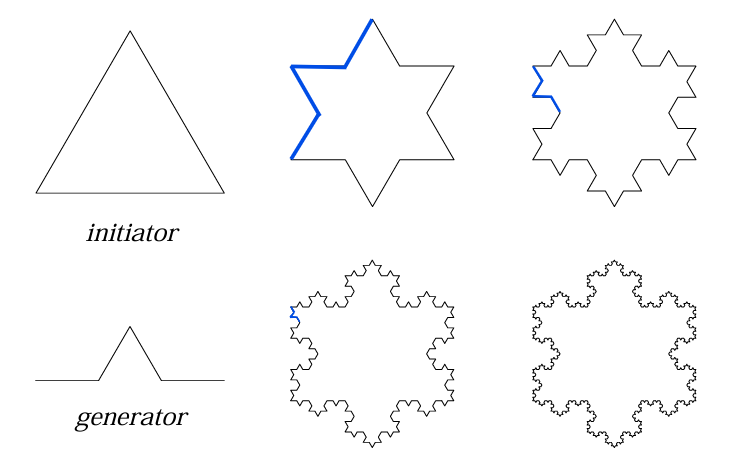
\includegraphics[width=12cm]{koch_curve} 
}
\caption{\label{fig:koch_curve} Construction of the Koch snowflake curve.~\cite{PRU:1990}}
\end{figure}

This functionality differs from traditional grammars as most systems based around them carry out rewriting sequentially. So, for example~\cite{EOM:2023}, if a character \textit{S} is to be replaced with the string \textit{SS} and you are starting with the axiom \textit{S}, the resulting string, both with sequential rewriting and parallel, would be \textit{SS}. But in the next generation, traditional grammars would give us the string \textit{SSS}, while l-system rewriting would give us \textit{SSSS} as all characters would be rewritten at once. While most self-similar structures can be replicated easier with l-systems because of this property, in instances where the first outcome(\textit{SSS}) is required, they would not be feasible.

\section{Aims \& Objectives}

The final product is expected to have a GUI-based L-system environment. The aim is to have options to generate different fractals and different kinds of plant-like structures. There would be an animated output that would show a certain number of generations while translating itself in such a way that the relative position of the productions remains the same and altering the length of rewritten lines so the relative size of the figure also remains somewhat constant. 

There are several potential implementations to demonstrate plant mimics, one of which has been implemented. The current implementation explores non-stochastic implementation and presents an output that branches in a very organic manner despite having no variation or randomness encoded in the rewriting rules. A step in the future would be to implement variation to have yet more realistic graphics. This would require some alteration to the current code to allow for multiple outcomes with varying probability instead of the existing setup with singular, predefined rules.

A further extension that is not required but I hope to implement is an option for user input that allow the user to select from a few predefined rule sets and then produce generations from a custom axiom that they set.

\section{Motivation}

The primary motivation in selecting this project topic was to understand the mathematics behind L-system productions and explore ways of translating string input into graphical output. There are several models online that allow customization of L-systems of varying complexity. Different variations have been developed using various other programming languages and frameworks, and allow different levels of customization to the user. This product will be written mainly in Java with imported libraries used where necessary.

The endeavour with this project, is to focus on plant structures and encode a level of randomness within the rewriting to present the user with a more realistic graphic that shows the progress of organic growth using a mix of preset and probability-based outcomes. The increasing complexity of graphical output provides a challenge that is compelling to research and understand. It requires learning new software and frameworks to see what implementation achieves the desired product to the highest degree of accuracy.

Some personal motivations were to create implementations that could map fossil-like objects. During initial research, before even finalizing the project choice, I came across a research paper that made use of L-systems to try and rebuild a fossil structure to study in detail and in doing so, realized the intricacy of the long-gone organisms~\cite{JHC:2014}. A personal objective immediately became to further develop my application in order to produce graphics resembling common fossils or shells. The fossils mentioned in the paper | rangeomorphs | have structures similar to ferns so the overall generations are still plant-like, but the implementations I hope to explore are more like ammonite fossils. I have seen productions of 3D L-systems that look similar~\cite{PAL:2008}, so I am confident that I can get to that production eventually.

\section{Milestones}

The progress over the course of this term has not been ideal. While most milestones set for Term 1 have been achieved, the timeline those achievements followed was not as expected. There was a large stretch of time where I was unable to make any progress with code due to ongoing assignments and exams. I was able to continue research in this time in small increments, but the progress was not significant and I did not get the chance to add these times to the project diary as there was no overall gain towards the project. 

Of the expected Term 1 milestones, I have been able to implement non-stochastic L-systems and carry out various research to understand different uses of L-system within different industries and professions. Findings on the classes of L-systems and some simple worked examples will be covered in section 2.1. 

The aim to also have some stochastic implementations functional was halted due to the nature of the current graphical output. I am currently unable to stage the outputs in a way that has them appearing one after the other. Due to this, the current output window is static and has all the structures appear simultaneously without any clear demonstration of progress. I decided to have several productions drawn on the final window so the progress of generations would be visible in some way still.
\newline

\textbf{\Large{Winter Break}}

While it is understood that no work is required over winter break, trials with different UI implementations will be carried out over the winter break in order to keep any persisting issues from delaying the timeline further. As there is still a lack of confidence in creating a fully functional GUI with Processing, a potential second consideration lies with JavaFX. Experimenting with different UI frameworks and software will allow for better understanding of the program, and will provide greater control with the visual output and how it is setup in the window. No explicit timeline will be set for this duration as greater flexibility can be granted for the duration of the break without affecting workflow in its entirety.

\textbf{\Large{Term 2}}

Ideally, if research and experimentation over winter break proves fruitful as expected, progress on the rest of the project should remain on track. I have allocated some time towards working on the recommended extensions, but this may prove difficult once the next term's coursework begins. 
\renewcommand{\arraystretch}{1.5}

\begin{longtable}{c|p{12cm}}
    Week beginning\\
    \hline

    20th January & Begin work on stochastic implementation. Have functional graphics ready by end of week\\
    27th January & Research and begin implementing GUI beyond simple rendering. Have semi-functional GUI by end of week\\
    3rd February & Begin compiling final report draft and continue work on GUI\\
    17th February & Have GUI fully functional and begin research on advanced plant mimics (consider context-sensitive implementation). Review progress with Anand\\
    24th February & Begin work on plant mimics and have functional for rendering by end of week\\
    3rd March & Take the week to review and work on report draft. Have users experiment with the UI and alter functionality where necessary\\
    10th March & Research 3D implementation and software or libraries needed for it if existing system cannot manage\\
    17th March & Begin 3D implementation and update report draft with findings\\
    24th March & Complete draft of final report and review with Anand\\
    31st March & Complete final report and submit\\
\end{longtable}

\chapter{Background Theory}

Before considering any kind of code implementation, it is important to understand the concept behind the different kinds of L-systems and how these distinctions affect the output. L-systems, while initially created to model plant growth, are incredibly efficient with self-similar fractals~\cite{MAN:1982} as well. In both cases, the parallel operation of L-systems is what makes them so successful. L-systems can broadly be classified using two axes: (1) deterministic or stochastic, and (2) context-free or context-sensitive~\cite{NANA:2010}. We explore here, the difference between deterministic and stochastic models.

\section{D0L-Systems}

The simplest class of L-systems are called D0L-systems (deterministic context-free L-systems). This is the kind of L-system that results in the commonly seen self-similar fractals. In the context of this class of L-system, there are individual rules corresponding to a character. To understand better, we can explore an example. 
\newline

\begin{figure}[h]
    \centering
	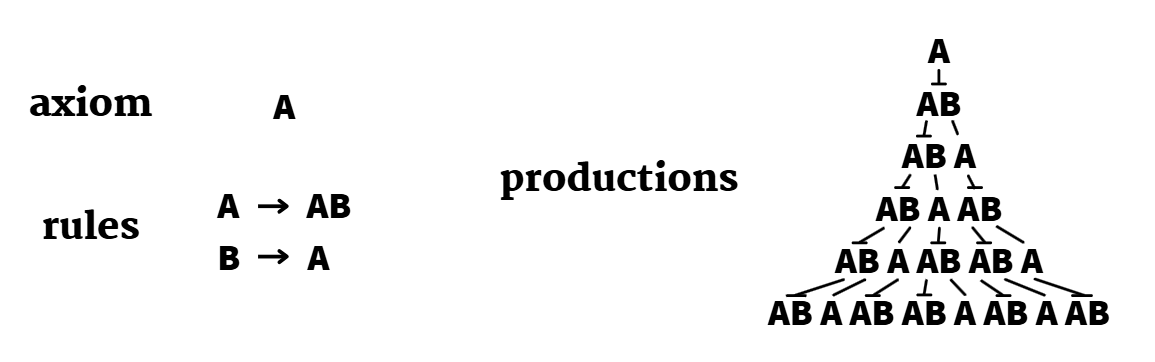
\includegraphics[width=14cm]{image.png} 
    \caption{\label{fig:image} Example of a derivation in a D0L-system.}
\end{figure}

We can consider strings built of two letters, $A$ and $B$. For each letter we specify a rewriting rule. In this case, $A \rightarrow AB$, and $B \rightarrow A$. This means that at each generation, every occurrence of $A$ will be rewritten with $AB$ and every occurrence of $B$ will be rewritten with $A$. We see this rewriting occur simultaneously across all $A$ and $B$ in each string production. Image generation with this class of L-system is also demonstrated in the introduction in Figure 1.1. 
\newline

\begin{figure}[!h]
    \begin{minipage}[c]{0.5\linewidth}
        \centering
        (a)
        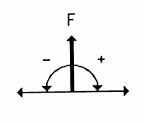
\includegraphics[width=4.5cm]{turtle.png}
    \end{minipage}\hfill
    \begin{minipage}[c]{0.5\linewidth}
        \centering
        (b)
        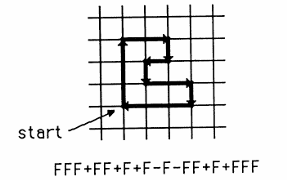
\includegraphics{turtlegrid.png}
    \end{minipage}
    \caption{(a) Turtle interpretation of string symbols F, +, -. (b)Interpretation of a string. The angle increment $\theta$ is equal to $90^{\circ}$. The turtle faces up initially~\cite{HAN:1989}.}
\end{figure}
\newpage

There have been countless extensions of the basic D0L-system model to create more complex fractals. We can see this with an approximation of the "quadratic Koch Island", beginning with the axiom $F+F+F+F$, and the production rule $F \rightarrow F+F-F-FF+F+F-F$. 

\begin{figure}[h]
    \centering
	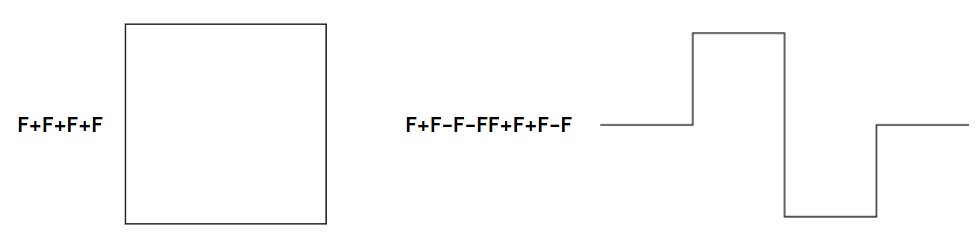
\includegraphics[width=15cm]{kochRule.png} 
    \caption{\label{fig:image} Koch Island axiom and rule}
\end{figure}

The following images correspond to the strings obtained in derivations of length 1-3, with the first image of Figure 2.3 being the image for derivation of length 0. The angle increment $\theta$ for this structure is $90^{\circ}$. The length of the straight line drawn is decreased with each generated image. This makes the distance between the endpoints of the polygon represented by the production successor equal to the length of the line of the line represented by the predecessor.

\begin{figure}[h]
    \centering
	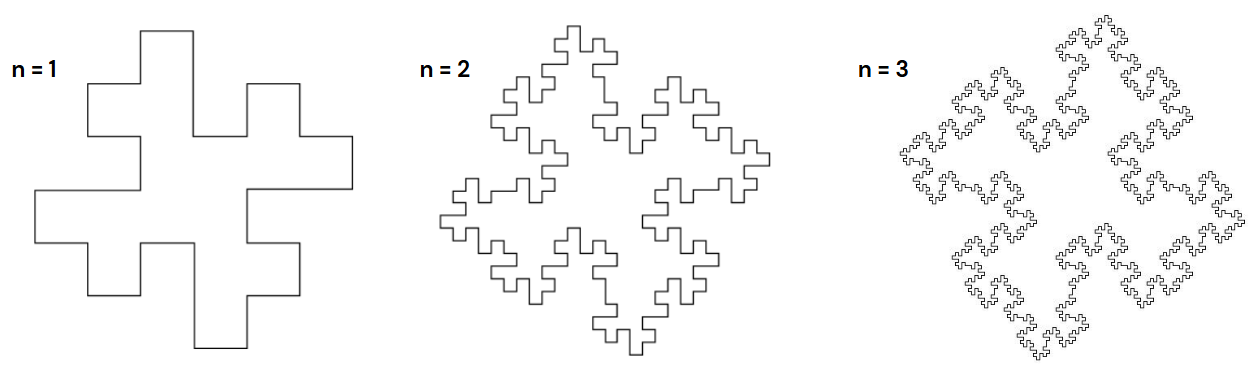
\includegraphics[width=15cm]{kochIsle.png} 
    \caption{\label{fig:image} Koch Island generations 1-3}
\end{figure}

Fractal images are customary with D0L-systems due to their strict rewriting, but these can also produce plant-like images to a high degree of accuracy. This is done using the characters "$[$" and "$]$". The $[$ saves the current position and moves according to the next command and, in doing so, branching off from the main structure. The $]$ then returns the turtle object back to the original position stored by the symbol "$[$".

\begin{figure}[h]
    \centering
	
\includegraphics[width=15cm]{D0Lplant.png} 
    \caption{\label{fig:image} Fractal tree using D0L-system with $\theta$ = $25^{\circ}$} Axiom: F, Rule $F \rightarrow FF-[-F+F+F]+[+F-F-F]$
\end{figure}

\section{Stochastic L-Systems}

Stochastic L-systems (S0L-systems | stochastic context-free L-systems) have the same main components of L-systems. The distinction from D0L-systems lies in the production rules and the way they are used. Stochastic L-systems integrate an extent of randomness into the produced models. Consequently, different graphical outputs can be obtained in simulations even if the initial conditions are identical for each run. The amount and direction of variation in the results depends on the chosen probability distribution that imposes structure on the simulation algorithms~\cite{PAL:2008}.

We can explore a simple example with the following rules:

\begin{center}
\begin{minipage}[c]{5cm}
    \flushleft
    $\omega : F$\newline
    $p_1 : F \xrightarrow{.33} F[+F]F[-F]F$\newline
    $p_2 : F \xrightarrow{.33} F[+F]F$\newline
    $p_3 : F \xrightarrow{.34} F[-F]F$
\end{minipage}
\end{center}

The production probability of each outcome is mentioned above the derivation symbol $\rightarrow$. Each production has a roughly 1/3 chance of being selected for the rewriting at every point of generation. The productions made using these rules are presented in Figure 2.6. Each of these figures begins with the same axiom. All lines drawn are of the same unit length and use the same angle of rotation at branching points, yet we can see numerous differences in each of the final products.
\newline

\begin{figure}[h]
    \centering
	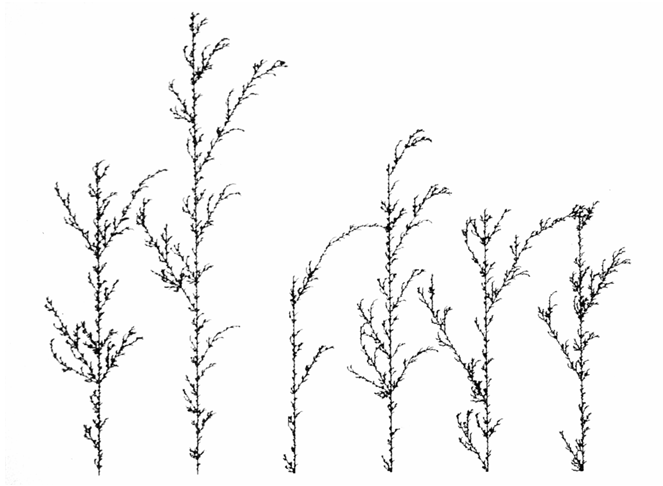
\includegraphics[width=14cm]{Stochplant.png} 
    \caption{\label{fig:image} Stochastic branching productions~\cite{PRU:1990}.}
\end{figure}

S0L-systems are most commonly used to mimic biological structures due to the controlled ambiguity that they allow within productions. They provide the opportunity to create different classes of plants, all sharing overall similar characteristics but differing in minor details. The plants in Figure 2.7 appear very similar yet are not identical.~\cite{ASH:1994}.

\begin{figure}[h]
    \centering
	
\includegraphics[width=14cm]{Stoch2.png} 
    \begin{center}
        \begin{minipage}[c]{5cm}
            $\omega : F$, $\theta : 22.5^{\circ}$\newline
            $p_1 : F \xrightarrow{.50} F[+F][-F]F$\newline
            $p_2 : F \xrightarrow{.30} F[-F]F$\newline
            $p_3 : F \xrightarrow{.20} F[+F]F$
        \end{minipage}
    \end{center}
    \caption{\label{fig:image} Three objects produced using stochastic L-systems.}
\end{figure}

We can see how minor differences in the rules and probabilities can change the final outcome drastically. The rules used for the images in Figures 2.6 and 2.7 are not dissimilar, yet the productions are completely different and would not fit in the same fictitious class of plants.

\section{Literature Survey}

I have gone through upward of a dozen research papers based on and around L-systems to gain better understanding on the topic. Depending on the reason for research, the papers discuss L-system in varying detail with every paper citing the most significant sources: \emph{Algorithmic Beauty of Plants~\cite{PRU:1990}}, and \emph{Lindenmayer Systems, Fractals, and Plants~\cite{HAN:1989}}. The former is a book written mainly by Aristid Lindenmayer and Przemyslaw Prusinkiewicz, the latter is a volume of the Springer book series \emph{Lecture Notes in Biomathematics~\cite{SPR}} . Both sources have similar material, though where the book focuses on modeling and analyzing plant growth progression, the volume on lecture notes presents some other avenues as well. 

Majority of papers using L-systems in different kinds of research begin with D0L-systems and then proceed to more complex applications by adding context-sensitive aspects. The papers all use somewhat algebraic notation to define L-systems and provide \emph{proof}, though these notations are not ones I understand quite so well yet. Those considering mathematical proofs, do not always compute graphical demonstrations, although the theories of those proofs are occasionally seen in use elsewhere. 

I will endeavour to better understand the mathematical proofs as I continue developing the application. 

\chapter{Current Progress}

The implementation of L-systems requires a way to rewrite strings according to the rules corresponding to specific characters, and a way to translate the resulting strings into graphical output. The implementation so far has been accomplished using an object-oriented approach. The main defined objects are:
\begin{itemize}
    \item a Rule object
    \begin{itemize}
        \item stores a character and its corresponding production string
        \item contains getters for both character and string attributes
    \end{itemize}
    \item an LSystem object
    \begin{itemize}
        \item initialized with an axiom and a \verb|List| of Rule objects
        \item getter for sentence as that is the only attribute accessed outside of the object
        \item checks if axiom has any characters outside the set alphabet and initializes the L-system with this string
        \item checks if a character has a production rule corresponding to it
        \item creates generations by rewriting the string using the rule set
    \end{itemize}
    \item a Turtle object
    \begin{itemize}
        \item initialized with a length and angle value corresponding to the specific L-system it is made for
        \item translates the LSystem string passed through to it into graphical output using Processing commands
    \end{itemize}
\end{itemize}

The main executor in the current implementation is a class extending \verb|PApplet| which is the Processing class used to create Graphical User Interfaces. Implementing \verb|PApplet| in Java requires overwriting the \verb|setup()| and \verb|draw()| functions to execute what is required. Due to the way in which these functions work together, executing the code in its current state brings up a window that already has the polygons drawn. 

There does not seem to be a defined method or command that allows the window to clear the screen after a pause. A \verb|clear()| function call clears the screen from the beginning so the window returns empty regardless of where in the code the function call is placed (i.e. before or after the draw functions). There is also not a function or command to delay the execution of the next draw capability so the overall implementation needs some revision to perform as expected.


\chapter{Software Engineering}

The program in its current state necessitates the creation of separate objects for each fractal. This means that each type of fractal needs to have a separate LSystem object to store the rules and axiom, and a separate Turtle object to define the line length and angle to obtain the final images. The following figure shows the UML diagram for the current implementation of the program.
\newline

\begin{figure}[h]
    \centering
	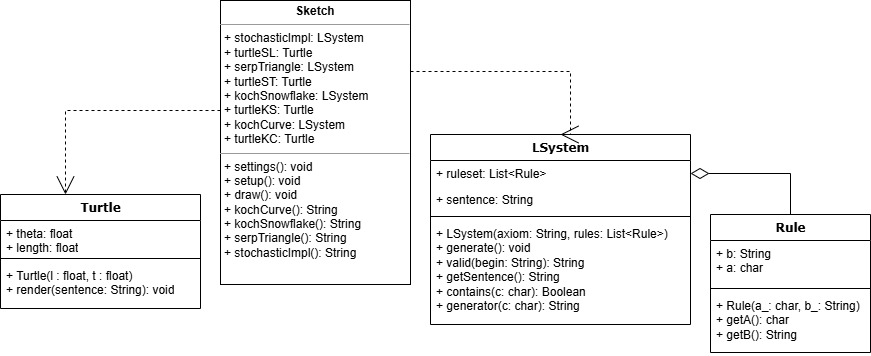
\includegraphics[width=16cm]{FYP_UML.jpg} 
    \caption{\label{fig:image} UML Diagram for current implementation}
\end{figure}

\section{Technological Choices}

The initial implementation has been accomplished using the \emph{Processing 4.3}~\cite{PRC} core library. This was selected due to its straightforward implementation of drawn graphics. The commands required to control output on a window are highly similar to traditional turtle graphics, a method used in most 2D implementations of L-systems and also the one depicted in the original sources~\cite{PRU:1990}~\cite{HAN:1989}. Using Processing with a defined \verb|Turtle| object | to account for the variation in line length and angle values | allows for easier generation of fractal images that have been previously defined using notation corresponding to turtle commands.

There is, however, an issue that arose with the use of Processing. Since Processing exists as an IDE with its own language that is closely based on Java but is still distinct in itself, the use of its core library in a Java program is not the most convenient. The current use of its functions needs to be carefully translated into Java as almost all resources for Processing make of use of it as an IDE. Not all the functionalities are proving to be as effective as expected and a greater level of understanding and control is required to be able to implement the specifics I am aiming for. Currently, I have found another extended Processing library~\cite{G4P} developed by an independent programmer that seems a promising fit, but further experimentation with it is required.

\section{Git Usage}

I made use of branches to keep parts of the project separate. My diaryUpdates branch has only diary entries. Fractals branch has all the main implementation of D0L-systems. A testing branch to keep the test and any edits made on that branch separate in case some error arises from the editing. I did, on occasion have to fetch files from different branches, namely the LSystem file from the testing branch after errors in the code were fixed. 

\section{Testing}

The majority of this project is graphics based so there is minimal testing for that at this time. There was testing carried out for the LSystem string generations, however. The tests ensured that rewriting was accurate and led to the addition of a method to check validity of starting input. 

Going forward, several more tests will need to be added as I begin to work on stochastic L-systems as the nature of their rewriting rules may cause issues during implementation. The probabilistic outcomes may prove troublesome to execute without extensive testing.

\chapter{Appendix}

\section{Diary}

\textbf{Lindenmayer Systems Project Diary}

Entry 12 - Dec 3rd

I have functional graphics for Koch Curve, Koch Snowflake, and Sierpinski Triangle. There was some issue in developing since Processing seems to not have any sort of delay that would allow one graphic to remain on the window for a set time before I can clear the screen and present the next one. Currently, compromised to have several iterations of each fractal so the progress of generations can be seen clearly with fractals of different complexities.

I might consider shifting from Processing to JavaFX since that seems to be a more reasonable avenue now that I have a better understanding of both and what exact functionalities they provide me with. Simpler fractals are easy to portray via the PApplet class, but as I progress, I would prefer to have better control of the output window.

Entry 11 - Dec 1st

I was right about where exactly the error was stemming from. Did a bit of testing to make sure the issue was sorted and added a validation method to make sure the input string doesn't have any undefined characters.

If undefined characters did make it through via the rules somehow, it should still be fine since the switch case in Turtle simply moves on as the default. This may come in handy if I end up taking user input later in term 2.

Entry 10 - Nov 29th

Attempted first LSystem implementation, not yet functional. I think there's some issue with the way the strings are being generated. I might need to change how I'm storing the rules. List might be better since there's separate components of the Rule objects that I need to access constantly. Maybe iterating by index might help. List.get() would be convenient for it.

Entry 09 - Nov 27th

I had some issues importing Processing as a library but managed a functional setup page extending PApplet. I've made a Turtle class to determine the initial default functionality of the turtle object. This will be the pen that determines sketch with the use of specific parameters. Some trial and error will be required to accurately implement fractal graphics.

I am considering adding a coded demonstration of the String multiplication but am unsure if it would be useful. I will have an example like this in my report regardless.

Entry 08 - Nov 23rd

Begun implementation of code. I've decided to use the processing library, so I can implement Turtle graphics as this is the most researched and easy to understand method in building functional L-systems.

Entry 07 - Oct 26th

I have added the LaTeX files for the project plan to the repo and have begun drafting the report.

Entry 06 - Oct 15th

I have been unable to upload the LaTeX file for my project plan onto IntelliJ. For now the pdf version is up and I will try again with LaTeX, but I am having issues with TeXiFy-IDEA despite having the necessary plugins. I will remove the pdf from the repo once the LaTeX issue is sorted as I edit those documents via Overleaf.
I have been reading The Algorithmic Beauty of Plants and the above-mentioned Lindenmayer Systems, Fractals, and Plants to get some reference on how to best show the working of the rewriting system.

Entry 05 - Oct 11th

Final draft of project plan completed and submitted. Java Swing and Processing noted as potential libraries for GUI; further research required. Had issues adding latex files to project repo, will attempt again later.

Entry 04 - Oct 9th

First draft completed and reviewed by supervisor. Begun edits.

Entry 03 - Oct 7th

First draft of project plan underway, expected completion by Tuesday afternoon for supervisor review.

Entry 02 - Oct 3rd

Started on book The Algorithmic Beauty of Plants and further related resources through algorithmicbotany.org

Noting On the Evolution of Parametric L-systems and Lindenmayer Systems, Fractals, and Plants as next sources to explore.Meeting with supervisor, discussed expectations for the project plan and questions about final project deliverables.

Entry 01 - Oct 2nd

I have an outline of the project plan set. Looked into research I can site. Found several helpful tutorials for guidance as well as a couple books and papers. Current research avenues: refseek, Semantic Scholar, Google Scholar.

\section{Video Demo}

\href{https://youtu.be/dCie_R_jZ4k}{Video Demo}

%%%% ADD YOUR BIBLIOGRAPHY HERE
\newpage
\begin{thebibliography}{99}
\addcontentsline{toc}{chapter}{Bibliography}
\bibitem{PRU:1990} Przemyslaw Prusinkiewicz and Aristid Lindenmayer. \emph{The Algorithmic Beauty of Plants}.  Springer-Verlag, New York, 1990.
\bibitem{EOM:2023} Grzegorz Rozenberg and Arto Salomaa. \emph{L-systems. Encyclopedia of Mathematics}. Springer, 2023.
\bibitem{MAN:1982} Benoit Mandelbrot. \emph{Fractal Geometry of Nature}. W.H. Freeman, 1982.
\bibitem{NANA:2010} Ryohei Nakano and Naoya Yamada. \emph{Number Theory-Based Induction of Deterministic Context-free L-system Grammar}. SciTePress, 2010.
\bibitem{HAN:1989} Przemyslaw Prusinkiewicz and James Hanan. \emph{Lindenmayer systems, fractals, and plants}. Springer-Verlag, Berlin, 1989.
\bibitem{JHC:2014} Hoyal Cuthill and Conway Morris. \emph{Fractal branching organizations of Ediacaran rangeomorph fronds reveal a lost Proterozoic body plan}. PNAS, Cambridge, 2014.
\bibitem{PAL:2008} Guillaume Dera, Gunther J. Eble, Pascal Neige, and Bruno David. \emph{ The flourishing diversity of models in theoretical morphology: from current practices to future macroevolutionary and bioenvironmental challenges}. CNRS Biogéosciences, Dijon, 2008.
\bibitem{ASH:1994} Ashok Samal, Brian Peterson and David J. Holliday. \emph{Recognizing Plants Using Stochastic L-systems}. IEEE, Texas, 1994.
\bibitem{SPR} Lecture Notes in Biomathematics. \emph{https://www.springer.com/series/0564}
\bibitem{PRC} Processing 4.3. \emph{https://processing.org/}
\bibitem{G4P} G4P. \emph{http://www.lagers.org.uk/g4p/index.html}
\end{thebibliography}
\label{endpage}



\end{document}
